\subsection{Boolean logic}

As the word ``digital'' suggests, digital computers operate on individual digits. In most modern machines, the base of these digits is 2, hence called ``binary'' numbers, where one digit is a binary digit or ``bit''. While there are computers using a trinary or even higher-valued number base \cite{wikipedia_setun}, the binary system has proven to be simple and robust to implement. In an electrical representation, a line pulled towards the GND potential represents a logical 0. Similarly, pulling the same line towards a predefined voltage level different from GND represents a logical 1. Due to their close association to electronic implementation, these logic levels are also called LOW and HIGH, respectively. Therefore, we define:

\begin{align}
    LOW  &\coloneqq 0       \\
    HIGH &\coloneqq 1       \\
    \mathcal{B} &= \{0, 1\} \\
    \mathcal{B}^2 &= \{00, 01, 10, 11\}  \\
    \mathcal{B}^n &= \cdots \nonumber
\end{align}

\subsubsection{Logical operators} \label{sec:logical_operators}

To do meaningful computation, logical operators are defined. Each operator is a function of one or more binary digit inputs, producing a single binary digit output. They have the shared signature $\mathcal{B}^n \to \mathcal{B} \mid n \geq 1$, where $n$ denotes the number of inputs. Since each input can only assume the state HIGH or LOW, for an operator taking $n$ inputs, there are $2^n$ combinations of input states. Therefore, there can only be $2^{2^n}$ different operators for any given $n$. For operators with $n = 2$, there are only 16 different mappings from inputs to outputs. Operators that have either one or two inputs can be written in infix notation. For this reason, many such operators have been given widely recognized names and symbols. \autoref{tab:boolean_operators} shows names and symbols of operators relevant to this paper. The order of the inputs of all given operators does not matter. For this reason, the inputs are unlabelled in their graphic representations later on.

\vspace{1em}
\begin{minipage}[t]{\textwidth}
    \centering
    \begin{tabular}{|c|c|c|c|c|c|c|c|} 
        \hline
        \textbf{A} & \textbf{B}   & \bm{$A \land B$} & \bm{$A \lor B$} & \bm{$A \lnand B$} & \bm{$A \lnor B$} & \bm{$A \lxor B$} & \bm{$\lnot A$}  \\ 
                   &              & AND              & OR              & NAND              & NOR              & XOR              & NOT             \\
        \hline
        0          & 0            & 0                & 0               & 1                 & 1                & 0                & 1               \\ 
        \hline
        0          & 1            & 0                & 1               & 1                 & 0                & 1                & 1               \\ 
        \hline
        1          & 0            & 0                & 1               & 1                 & 0                & 1                & 0               \\ 
        \hline
        1          & 1            & 1                & 1               & 0                 & 0                & 0                & 0               \\
        \hline
    \end{tabular}
    \label{tab:boolean_operators}
    \captionof{table}{Boolean operators}
\end{minipage}

The algebra defined by these logical operators is called "Boolean algebra". Expressions of this algebra can make use of named variables and parenthesis, as would be the case in regular algebra. By nesting and reusing functions in this language, any mapping of any number of inputs to any number of outputs can be denoted. There are rules on how operations can be transformed into different operations denoting the same logical mapping. For brevity, this set of rules is not explained here. An extensive overview of these transformations and their application is given in \cite{shannon1938symbolic}. Here is an example of an expression in this language:

\begin{displaymath}
    \neg(\neg A \land \neg B)
\end{displaymath}

A set of operators is called functionally complete if and only if its operators can be composed in a way that emulates all other operators of the same number of inputs. For 2 inputs, there are only 16 distinct operators. If a subset of operators can be used to compose all 16, it is deemed functionally complete, as it can be used to denote any logical function. Examples of such functionally complete sets include:

\begin{gather}
    \{AND, OR, NOT\} \label{gather_and_or_not} \\
    \{NAND\}         \\
    \{XOR, NOT\}
\end{gather}

Consider the expression given earlier, $\neg(\neg A \land \neg B)$. The outputs of the entire expression are identical to that of the OR gate. However, only the NOT and AND operators are used within the expression. Therefore, the set of operators given in set \ref{gather_and_or_not} is functionally complete, but not minimal, because the OR operator can be emulated by the AND and NOT operators. Thus, the OR can be dropped from the set, while retaining its functional completeness. A set of boolean operators is considered minimal when removing any operator causes the set to no longer be functionally complete. An even more restrictive category are the "Sheffer functions", which are also known as \textit{sole sufficient operators}. They are the functionally complete sets which contain only a single boolean operator. For operators with 2 inputs, there are only two such sets: $\{NAND\}$ and $\{NOR\}$.

\subsubsection{Logic gates}

Since most digital processors work using electrical circuits, there is a need for a notation that can be shared by electricians and logicians. Since all boolean operators as defined in \autoref{sec:logical_operators} produce only a single binary digit but take $n$ inputs, chaining multiple such operators naturally results in a logical tree structure. These trees can be drawn without intersections, as each tree is a planar graph\cite{West2001}. If a recursive connection is made, as is required for implementing memories, the non-recursive subtrees can still be drawn without intersections. Therefore, if boolean circuit contains an intersection, it also contains recursion. 

Each operator is assigned a unique symbol that is drawn at the respective graph edge. In real world applications, one operator corresponds to one or more physical components, which are collectively called a "logic gate". Figures \ref{fig:logic_gates_and} - \ref{fig:logic_gates_not} show the symbols used for the AND, OR and NOT gate defined in \autoref{tab:boolean_operators}. The symbols used are defined in standard 14456 by the \ac{ieee} \cite{STD14456}. The equivalent \ac{iso} standard that defines symbols for these functions is ISO 60617. \cite{ISO60617}.

\begin{figure}[H]
    \centering
    % First image
    \begin{minipage}{0.3\textwidth}
        \centering
        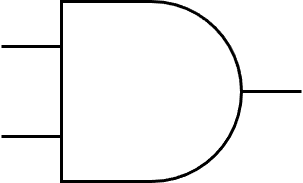
\includegraphics[width=0.7\textwidth]{images/drawio/and_symbol.png}
        \caption{AND Gate, defined in \cite{STD14456}}
        \label{fig:logic_gates_and}
    \end{minipage}
    \hfill
    % Second image
    \begin{minipage}{0.3\textwidth}
        \centering
        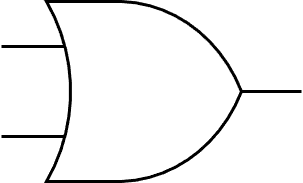
\includegraphics[width=0.7\textwidth]{images/drawio/or_symbol.png}
        \caption{OR Gate, defined in \cite{STD14456}}
        \label{fig:logic_gates_or}
    \end{minipage}
    \hfill
    % Third image
    \begin{minipage}{0.3\textwidth}
        \centering
        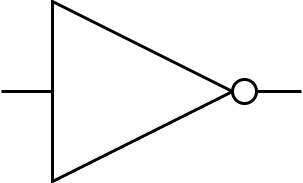
\includegraphics[width=0.7\textwidth]{images/drawio/not_symbol.png}
        \caption{NOT Gate, defined in \cite{STD14456}}
        \label{fig:logic_gates_not}
    \end{minipage}
\end{figure}

As an example for composition, consider the boolean expression given above, $\neg(\neg A \land \neg B)$. Its visual representation can be seen in \autoref{fig:or_from_and}. This representation allows electrical engineers to reason about the structure in terms of electrical connections and components, while logicians can easily convert it to its boolean algebra form. 

\begin{figure}[H]
    \centering
    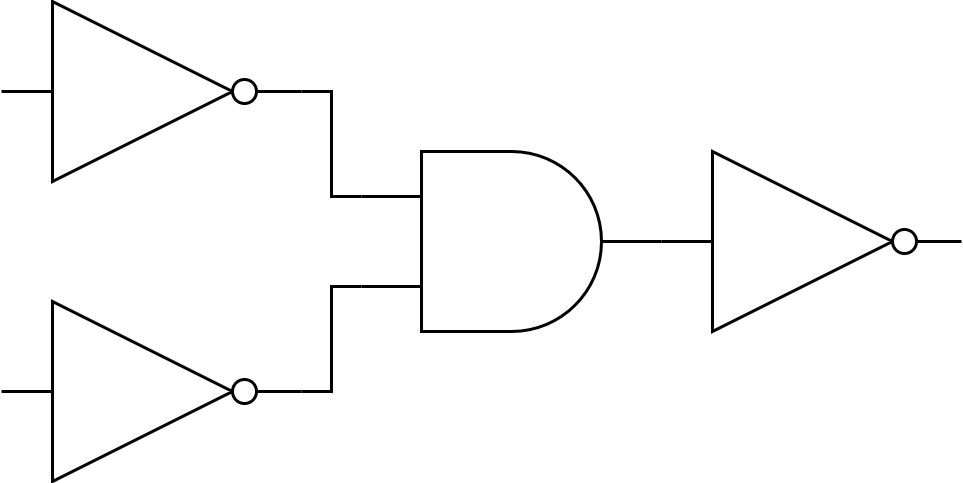
\includegraphics[width=0.7\textwidth]{images/drawio/or_from_and.png}
    \caption{Visual representation of $\neg(\neg A \land \neg B)$}
    \label{fig:or_from_and}
\end{figure}

\subsubsection{Multiplexer} \label{sec:fundamentals_boolean_logic_multiplexer}

A multiplexer is a commonly used circuit of logic gates used to select one of multiple inputs and propagate it to its output. To select between $n$ input signals, $\lceil log_2(n)\rceil$ selector signals are required. For example, two select between 3 different input signals, a selector signal of 2 bits is needed. If multiple multiplexers are operated in parallel and use the same selector signal, the set of multiplexers can be thought of as a single multiplexer with a data channel of $m$ bits. A multiplexer that switches between $n$ words of $m$ bits each is referred to as an ``m bit n:1 multiplexer''. All combinations of $n$ and $m$ can be built using only the basic 1 bit 2:1 multiplexer. Its output for the input signals $A$, $B$ and $S$ is determined by the boolean expression:

\begin{displaymath}
    (A \land \neg S) \lor (B \land S)
\end{displaymath}

\begin{figure}[H]
    \centering
    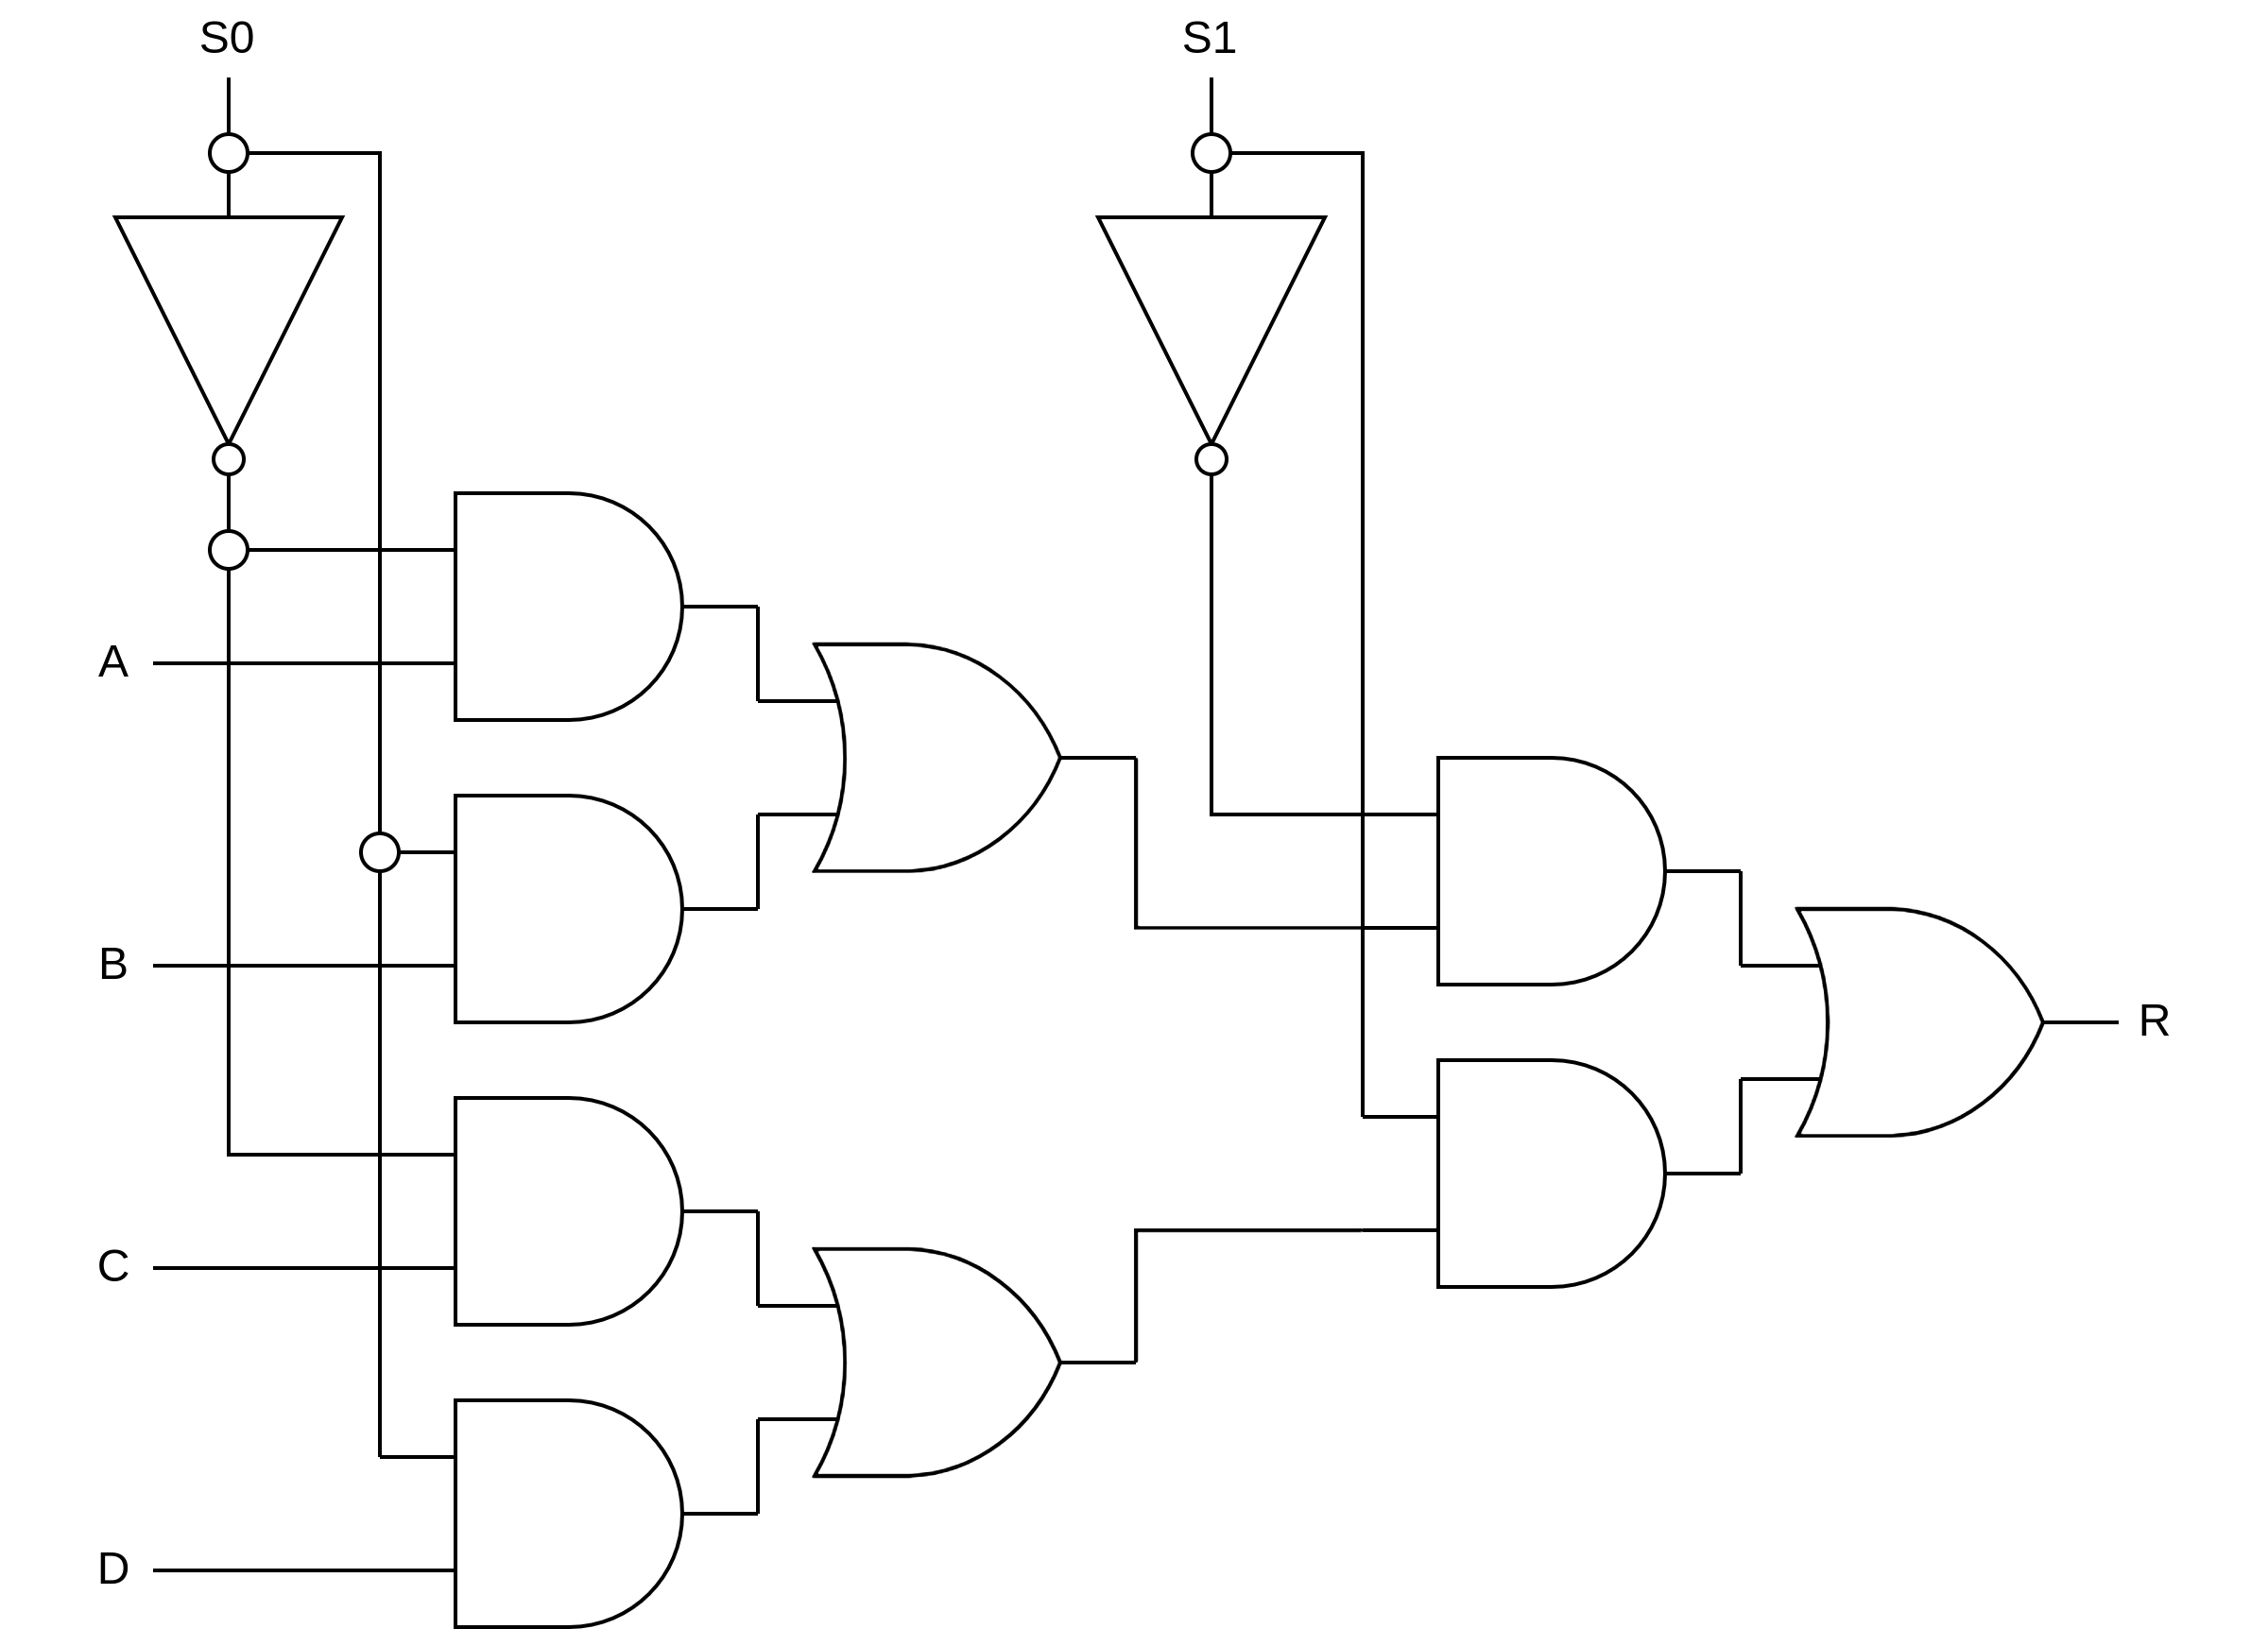
\includegraphics[width=0.7\textwidth]{images/drawio/multiplexer_tree.png}  % Replace with your image file
    \caption[4:1 multiplexer from three 2:1 multiplexers]{1 bit 4:1 multiplexer from three 1 bit 2:1 multiplexers}
    \label{fig:implementation_modularisation_multiplexer_tree}
\end{figure}

To increase the number of inputs that can be selected from, a tree of 2:1 multiplexers is created. In this tree, the inputs of the leaves are the inputs of the resulting combined multiplexer. Each layer of the tree uses one bit of the selection input signal. By constructing a multiplexer this way, multiplexers with an arbitrary number of inputs can be constructed, provided the number of inputs is a power of two. This is a direct representation of a binary tree, since each individual 2:1 multiplexer serves as a tree node with two children. To increase the word size of a multiplexer, multiple n:1 multiplexers can be operated in parallel, again sharing their selection input signals. \autoref{fig:implementation_modularisation_multiplexer_tree} shows a 1 bit 4:1 multiplexer built from three individual 1 bit 2:1 multiplexers. For a filled, unskewed binary tree, the number of leaf nodes for a tree of height $h$ is given by $2^{h + 1} - 1$ \cite{tanenbaum2012sco}. Since each leaf multiplexer has 2 inputs, for an $m$ bit multiplexer of $n$ inputs, the following equation gives the number of 1 bit 2:1 multiplexers required in total:

\begin{displaymath}
    N_{multiplexers}(n, m) = m \times (2^{\lceil log_2(n) \rceil} - 1)
\end{displaymath}

As an example, an 8 bit 4:1 multiplexer requires 
\begin{displaymath}
    N_{multiplexers}(4, 8) = 8 \times (2^{\lceil log_2(4) \rceil} - 1) = 24
\end{displaymath}

1 bit 2:1 multiplexers.
